\documentclass[11pt,oneside]{book}
\usepackage{enumitem}
\usepackage{fancyhdr}
\usepackage[a4paper,top=2cm,bottom=3cm,left=2cm,right=2cm,marginparwidth=1.75cm]{geometry}
\usepackage{eurosym}
\usepackage{hyperref}

%\usepackage[T1]{fontenc}
% For Vietnamese characters
\usepackage[T5]{fontenc}
\usepackage[utf8]{inputenc}

\usepackage{multicol}
\usepackage{pdfpages}
\BLOCK{if not nopax}
\usepackage{pax}
\BLOCK{endif}
\usepackage{times}
\usepackage[english,latin]{babel}


\usepackage{transparent}
\usepackage[
  firstpage=True,
  placement=center,
  angle=0,
  color=black!40,
  scale=1,
  hshift=0,
  vshift=0,
  opacity=1,
  position={7cm,-12cm}
  ]{background}

\hypersetup{
    colorlinks,
    linktoc=all,
    linkcolor=red,
}
\setlength{\paperwidth}{21cm}    % A4
\setlength{\paperheight}{29.7cm} % A4
\special{papersize=21cm, 29.7cm}
\pdfpageheight\paperheight
\pdfpagewidth\paperwidth
\setlength\topmargin{-5mm} \setlength\oddsidemargin{-0cm}
\setlength\textheight{24.7cm} \setlength\textwidth{16cm}
\setlength\columnsep{0.6cm}  \newlength\titlebox \setlength\titlebox{2.00in}
\setlength\headheight{5pt}   \setlength\headsep{0pt}
\setlength\footskip{1.0cm}
\setlength\parindent{0pt}

\pagestyle{plain}
\pagenumbering{roman}

\date{}
\title{ACL Anthology}

% General use macros
\BLOCK{macro committee_member(member)}\VAR{member.first_name} \BLOCK{if member.middle_name is defined}\VAR{member.middle_name} \BLOCK{endif}\VAR{member.last_name}\BLOCK{if member.institution is defined}, \VAR{member.institution}\BLOCK{endif}\BLOCK{endmacro}

\begin{document}

%%%%%%%%%
% Cover %
%%%%%%%%%
\begin{titlepage}

  %CenterWallPaper{1}{/Users/xilini/aclpub2_proceedings/resourceful-2023/prefaces/cover.jpg}
  \backgroundsetup{
            contents={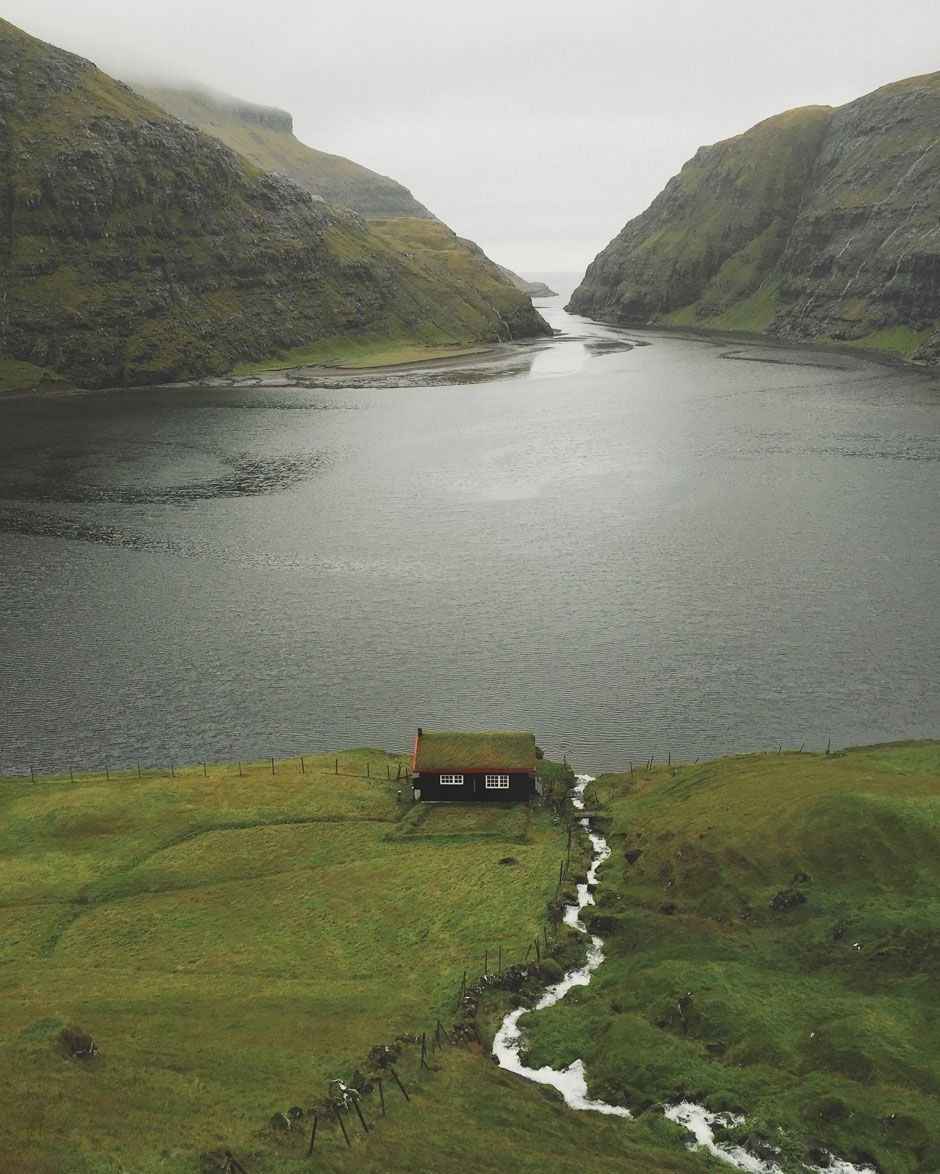
\includegraphics{/Users/xilini/aclpub2_proceedings/resourceful-2023/prefaces/faroe.jpg}}
        }
  
  \begin{center}
    \vspace{1.5cm}

    {\LARGE \textbf{\textcolor{white}{\VAR{conference.anthology_venue_id} \VAR{conference.start_date.year}}}}

    \vspace*{65mm}

    \vspace*{3cm}
    {\bf\huge \transparent{2}\textcolor{white}{\VAR{conference.event_name}}}

    \vspace*{1cm}

    {\bf\LARGE \textcolor{white}{\VAR{conference.cover_subtitle}}}

    \vfill
    \vspace*{6cm}

    {\LARGE \textcolor{white}{\VAR{conference_dates}, \VAR{conference.start_date.year}}}

    \vspace*{.5cm}

    {\LARGE \textcolor{white}{Tórshavn, Faroe Islands}}

    \vspace*{2cm}
    {\LARGE \textcolor{white}{Editors: Dana Dannélls, Simon Dobnik, Nikolai Ilinykh, Beáta Megyesi, Felix Morger, Joakim Nivre}}
    \vspace{-1cm}

  \end{center}
\end{titlepage}
\newpage

%%%%%%%%%%%%
% Sponsors %
%%%%%%%%%%%%
\BLOCK{if sponsors}
\setcounter{page}{2}
\vspace*{2cm}
\noindent

%{\Large The \VAR{conference.anthology_venue_id} organizers gratefully acknowledge the support from the following sponsors.}
%\bigskip

%\vspace*{1cm}

\BLOCK{macro generate_sponsor_tier(tier)}
  \begin{samepage}
  \noindent
  {\Large \textbf{\VAR{tier.tier}}}
    
  
  \nopagebreak
  \BLOCK{for logo_batched in tier.logos|batch(4)}
    \BLOCK{for logo in logo_batched}
      \begin{minipage}[c][0.4\linewidth][c]{0.21\linewidth}
        \includegraphics[width=\linewidth]{\VAR{root}/sponsor_logos/\VAR{logo}}
      \end{minipage}\hspace{0.2\linewidth}
    \BLOCK{endfor}
  \BLOCK{endfor}
  \end{samepage}
\BLOCK{endmacro}

\BLOCK{for tier in sponsors}
  \VAR{generate_sponsor_tier(tier)}
  \bigskip
  \bigskip
\BLOCK{endfor}
\newpage
\BLOCK{endif}


%%%%%%%%%%%%%
% Copyright %
%%%%%%%%%%%%%
\vspace*{11cm}
{\large

\noindent
\textcopyright \VAR{conference.start_date.year} \VAR{conference.publisher}\\

\vspace*{1cm}
\noindent
Front-cover photo: Sage Stephens(@storyofsage, https://www.instagram.com/p/BZOuVK8HkUO/)

\vspace*{1cm}
\noindent
Order copies of this and other ACL proceedings from:

\vspace*{1cm}
\begin{tabular}{p{1.5cm}l}
& Association for Computational Linguistics (ACL)\\
& 209 N. Eighth Street\\
& Stroudsburg, PA 18360\\
& USA\\
& Tel: +1-570-476-8006\\
& Fax: +1-570-476-0860\\
&{\tt acl@aclweb.org}\\
\end{tabular}

\vspace*{1cm}
ISBN \VAR{conference.isbn}
\vspace*{1cm}

Editors: \\Dana Dannélls, Simon Dobnik, Nikolai Ilinykh, Beáta Megyesi, Felix Morger, Joakim Nivre

}
\newpage


%%%%%%%%%%%%
% Prefaces %
%%%%%%%%%%%%
\BLOCK{if prefaces}
\BLOCK{for preface in prefaces}
  \begin{center}
   { \Large \textbf{\VAR{preface.title}}}
  \end{center}
  \vspace*{0.5cm}
  \VAR{load_file(root, "prefaces", preface.file)}
  \newpage
\BLOCK{endfor}
\BLOCK{endif}

%%%%%%%%%%%%%%%%%%%%%%%%
% Organizing Committee %
%%%%%%%%%%%%%%%%%%%%%%%%
\BLOCK{if organizing_committee}
\begin{center}
{\Large \textbf{Organizing Committee}}
\end{center}
\vspace*{1cm}
\begin{description}
\BLOCK{for role in organizing_committee}
  \item{\bf \VAR{role.role}}\vspace{2mm}\\
  \BLOCK{for member in role.members}
    \VAR{committee_member(member)}\\
  \BLOCK{endfor}
\BLOCK{endfor}
\end{description}
\newpage
\BLOCK{endif}

%%%%%%%%%%%%%%%%%%%%%
% Program Committee %
%%%%%%%%%%%%%%%%%%%%%
\BLOCK{if program_committee}
\begin{center}
\Large \textbf{Program Committee}
\end{center}
\vspace*{1cm}
\begin{description}
\BLOCK{for block in program_committee}
  \item{\bf \VAR{block.role}}\vspace{2mm}\\
  \BLOCK{if block.entries[0].area}
    \BLOCK{for area in block.entries}
      \emph{\VAR{area.area}}\\
      \BLOCK{if area.members[0].institution}
        \BLOCK{for member in area.members}
          \VAR{committee_member(member)}\\
        \BLOCK{endfor}
      \BLOCK{endif}
      \BLOCK{if not area.members[0].institution}
        \VAR{join_name(", ", area.members)}\\
      \BLOCK{endif}
    \BLOCK{endfor}
  \BLOCK{elif block.type is equalto("name_block")}
    \BLOCK{for name_block in group_by_last_name(block.entries)}
      \VAR{join_names(", ", name_block)}\\
      \newline
    \BLOCK{endfor}
  \BLOCK{elif block.type is equalto("name_block_without_newlines")}
    \VAR{to_string_sorting_by_last_name(block.entries)}\\
    \newline
  \BLOCK{else}
    \BLOCK{for member in block.entries}
      \VAR{committee_member(member)}\\
    \BLOCK{endfor}
  \BLOCK{endif}

\BLOCK{endfor}
\end{description}
\newpage
\BLOCK{endif}

%%%%%%%%%%%%%%%%%
% Invited Talks %
%%%%%%%%%%%%%%%%%
\BLOCK{if invited_talks}
\BLOCK{for talk in invited_talks}
  \begin{center}
    {\LARGE \textbf{Keynote Talk: \VAR{talk.title}}\\}
    \vspace*{0.5cm}
    %\begin{minipage}[c][0.35\linewidth][c]{0.35\linewidth}
     % \end{minipage}\\
    \textbf{\VAR{talk.speaker_name}}\\
    \BLOCK{if talk.institution}
    \VAR{talk.institution}\\
    \BLOCK{endif}
    
    \BLOCK{if talk.photo}
   \begin{center}
        \includegraphics[width=0.3\linewidth]{\VAR{root}/invited_talks/\VAR{talk.photo}}
     \end{center}    
    \BLOCK{endif}
    
    \BLOCK{if talk.date}
    \textbf{\VAR{talk.date}} -- 
    \BLOCK{endif}
    \BLOCK{if talk.time}
    Time: \textbf{\VAR{talk.time}} --
    \BLOCK{endif}
    \BLOCK{if talk.location}
    Room: \textbf{\VAR{talk.location}}\\
    \BLOCK{endif}
    
  \end{center}

  \vspace*{0.2cm}
  \BLOCK{if talk.abstract_file}
  \textbf{Abstract:} \VAR{load_file(root, "invited_talks", talk.abstract_file)}\\
  \newline
  \BLOCK{endif}

  \BLOCK{if talk.bio_file}
  \textbf{Bio:} \VAR{load_file(root, "invited_talks", talk.bio_file)}
  \newpage
  \BLOCK{endif}
\BLOCK{endfor}
\BLOCK{endif}


%%%%%%%%%%%%%%%%%
% Panels %
%%%%%%%%%%%%%%%%%
\BLOCK{if panels}
\BLOCK{for panel in panels}
  \begin{center}
    {\LARGE \textbf{Panel: \VAR{panel.title}}}
    
    \BLOCK{if panel.photo}
        \begin{center}
        \includegraphics[width=\linewidth]{\VAR{root}/panels/\VAR{panel.photo}}
        \end{center}
    \BLOCK{endif}
    
    \vspace*{0.5cm}
    \BLOCK{if panel.date}
    \textbf{\VAR{panel.date}} -- 
    \BLOCK{endif}
    \BLOCK{if panel.time}
    Time: \textbf{\VAR{panel.time}} --
    \BLOCK{endif}
    \BLOCK{if panel.location}
    Room: \textbf{\VAR{panel.location}}
    \BLOCK{endif}
  \end{center}
  \BLOCK{if panel.abstract_file}
  \VAR{load_file(root, "panels", panel.abstract_file)}\\
  \BLOCK{endif}
  \newline
    %\begin{minipage}[c][0.35\linewidth][c]{0.35\linewidth}
     % \end{minipage}\\
    \BLOCK{if panel.moderators} 
    	\BLOCK{for moderator in panel.moderators} 
    	    \BLOCK{if moderator.name}
    			\textbf{\textbf{Moderator: }\VAR{moderator.name}},
    		\BLOCK{endif}
    		\BLOCK{if moderator.institution}
    		 	\textbf{\VAR{moderator.institution}}
    		\BLOCK{endif}
    		\BLOCK{if moderator.bio_file}
  				\VAR{load_file(root, "panels", moderator.bio_file)}\\

  			\BLOCK{endif}
    		 
    	\BLOCK{endfor}
    \BLOCK{endif}  
    
    \BLOCK{if panel.panelists} 
        \textbf{Panelists: }\\
    	\BLOCK{for panelist in panel.panelists} 
    	    \BLOCK{if panelist.name}
    			\textbf{\VAR{panelist.name}},
    		\BLOCK{endif}
    		\BLOCK{if panelist.institution}
    		 	\VAR{panelist.institution}
    		\BLOCK{endif}
    		\BLOCK{if panelist.bio_file}
  				\VAR{load_file(root, "panels", panelist.bio_file)}\\
  				\newline

  			\BLOCK{endif}
    		 
    	\BLOCK{endfor}
    \BLOCK{endif}


  \newpage
  
\BLOCK{endfor}
\BLOCK{endif}

%%%%%%%%%%%%%%%
% Special Additional Pages %
%%%%%%%%%%%%%%%
\BLOCK{if additional_pages}
\BLOCK{for additional_page in additional_pages}
  \begin{center}
   { \LARGE \textbf{\VAR{additional_page.title}}}
  \end{center}
  \vspace*{0.5cm}
  \VAR{load_file(root, "additional_pages", additional_page.file)}
  \newpage
\BLOCK{endfor}
\BLOCK{endif}

%%%%%%%%%%%%%%%%%%%%%
% Table of Contents %
%%%%%%%%%%%%%%%%%%%%%
\BLOCK{if archival_papers}
\newpage  % Empty page before TOC
\pagestyle{plain}
\begin{center}
{\Large \textbf{Table of Contents}}
\end{center}
\vspace*{1em}
\newcommand\page[1]{\rightskip=25pt \dotfill\rlap{\hbox to 25pt{\hfill#1}}\par}
\begin{itemize}[leftmargin=*,label={}]
  \BLOCK{for paper in archival_papers}
     \item \hyperlink{page.\VAR{paper.start_page}}{\emph{\VAR{paper.title}}}\\ \hspace*{2em} \VAR{join_names(", ", paper.authors, " and ")}\dotfill \hyperlink{page.\VAR{paper.start_page}}{\VAR{paper.start_page}}
  \BLOCK{endfor}
\end{itemize}
\newpage
\BLOCK{endif}

%%%%%%%%%%%
% Program %
%%%%%%%%%%%
\BLOCK{if program}
\renewcommand{\baselinestretch}{0.87}
\setlength{\parindent}{0in}
\setlength{\parskip}{2ex}

\begin{center}
{\Large \textbf{Program}}
\end{center}
\vspace*{0.5em}

\BLOCK{for date, pages in program}
  \BLOCK{set ns = namespace(first=true)}
  \BLOCK{for page in pages}
    \begin{tabular}{p{24mm}p{124mm}}
    \multicolumn{2}{l}{\bf \VAR{program_date(date)} \BLOCK{if ns.first is not true}(continued)\BLOCK{endif}} \\\\
    \BLOCK{for entry in page}
      \BLOCK{if entry.type is equalto("header")}
      \VAR{session_times(entry)} & \emph{\VAR{entry.title}}\\\\
      \BLOCK{endif}

      \BLOCK{if entry.type is equalto("paper")}
        \BLOCK{set paper = id_to_paper[entry.paper.id]}
        & \hyperlink{page.\VAR{paper.start_page}}{\emph{\VAR{paper.title}}}\\
        & \VAR{join_names(", ", paper.authors, " and ")}\\\\
      \BLOCK{endif}
    \BLOCK{endfor}
    \end{tabular}
    \newpage
    \BLOCK{set ns.first = false}
  \BLOCK{endfor}
\BLOCK{endfor}
\BLOCK{endif}

\BLOCK{if include_papers}  % Flag to generate only front matter or include papers.
%%%%%%%%%%
% Papers %
%%%%%%%%%%
\pagenumbering{arabic}
\setcounter{page}{1}
 \renewcommand{\headrulewidth}{0pt}
\BLOCK{for paper in archival_papers}
\phantomsection
  \addcontentsline{toc}{section}{\emph{\VAR{paper.title}}}
  \AddToShipoutPicture*{
    \setlength{\unitlength}{1mm}
    \footnotesize

    \BLOCK{if conference.watermark_book_title}
    \BLOCK{set title=conference.watermark_book_title}
    \BLOCK{else}
    \BLOCK{set title=conference.book_title}
    \BLOCK{endif}

    \put(0,13){\parbox[t]{\paperwidth}{\centering
    							\emph{Proceedings of the Second Workshop on Resources and Representations for Under-Resourced Languages and Domains} \\ \emph{(RESOURCEFUL-2023)},  pages \VAR{paper.start_page}--\VAR{paper.end_page}, \VAR{conference_dates}, \VAR{conference.start_date.year} \textcopyright
  							\VAR{conference.start_date.year} Association for Computational Linguistics}}
  }
  \includepdf[pagecommand={\thispagestyle{plain}},pages=-]{\VAR{root}/papers/\VAR{paper.file}}
\BLOCK{endfor}

%%%%%%%%%%%%%%%%
% Author Index %
%%%%%%%%%%%%%%%%
\begin{huge}
Author Index
\end{huge}
\vspace*{1em}
\begin{multicols}{2}
\BLOCK{for _, author_to_pages in alphabetized_author_index}
\BLOCK{for author, pages in author_to_pages}
\VAR{author}, \VAR{join_page_numbers(pages)}\\
\BLOCK{endfor}
\\ % Extra space between new letters.
\BLOCK{endfor}
\end{multicols}

\BLOCK{endif}

\end{document}
